\documentclass[a4paper]{article}
\usepackage[letterpaper, margin=1in]{geometry} % page format
\usepackage{listings} % this package is for including code
\usepackage{graphicx} % this package is for including figures
\usepackage{amsmath}  % this package is for math and matrices
\usepackage{amsfonts} % this package is for math fonts
\usepackage{hyperref} % for urls


\title{My first Document}
\date{2013-09-01}
\author{Morgan Baker}
\begin{document}
\lstset{language=Python}
	
\maketitle

\section{Solution to Section 1: Instructions}
The LaTeX platform is installed on the machine. Go to Figure \ref{fig:LaTeXConfirm} for picture proof.

\begin{figure}
  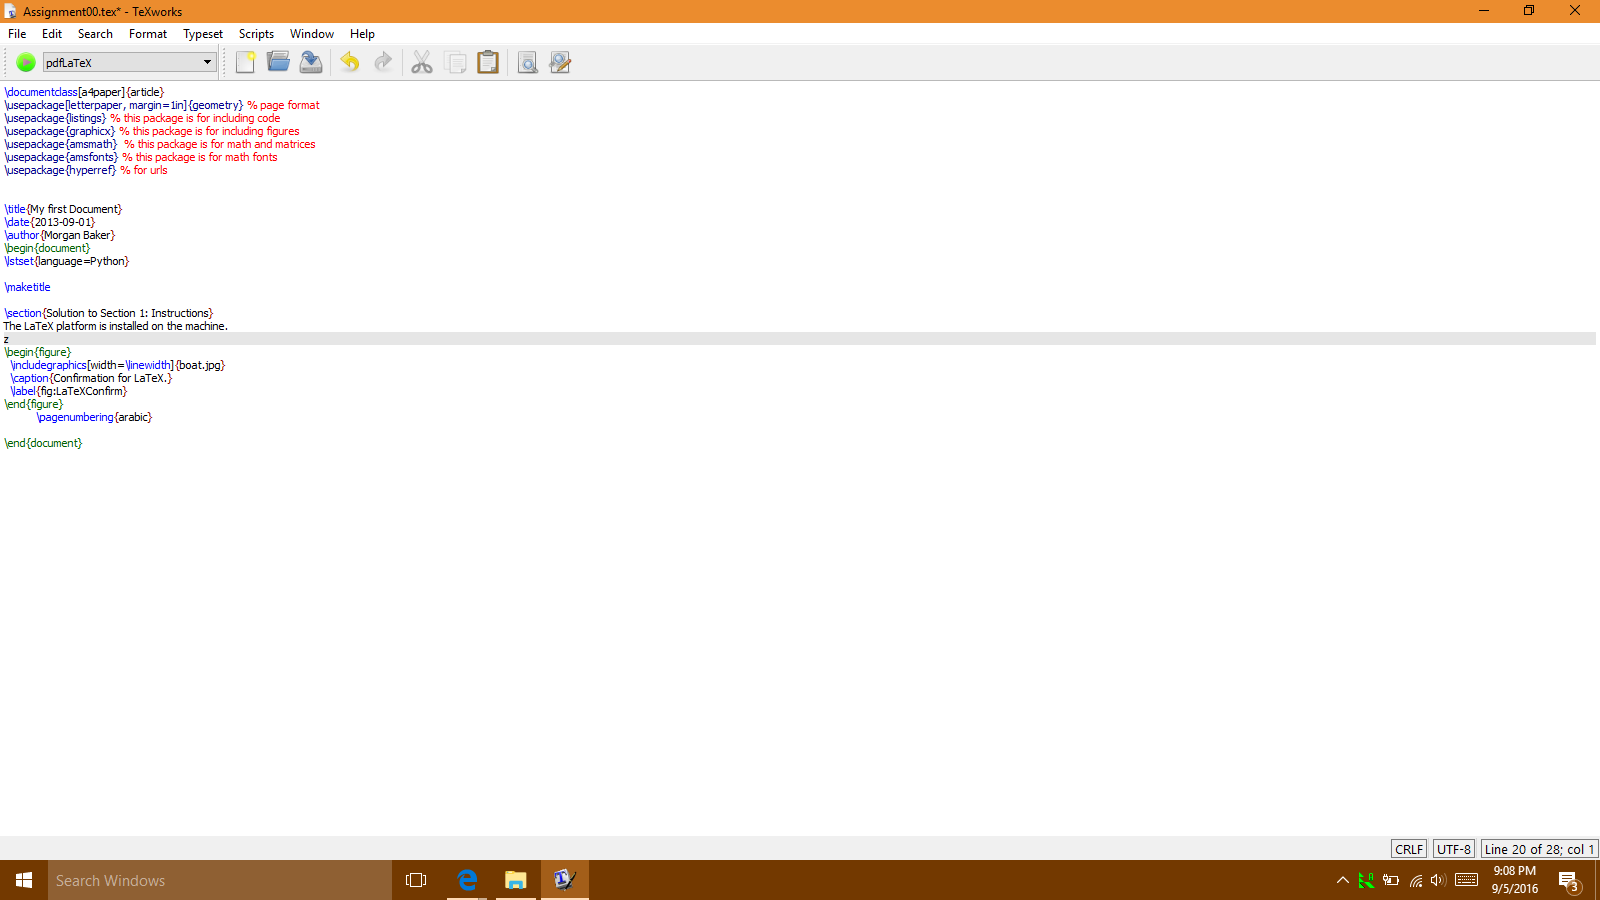
\includegraphics[width=\linewidth]{LaTeXConfirm.png}
  \caption{Confirmation for LaTeX.}
  \label{fig:LaTeXConfirm}
\end{figure}

\section{Solution to Section 2: Course Setup}
\subsection{Solution to Section 2.1}
Python has been installed. Take a look at Figure \ref{fig:PythonConfirm} for picture proof, and Confirmation.py for the code.

\begin{figure}
  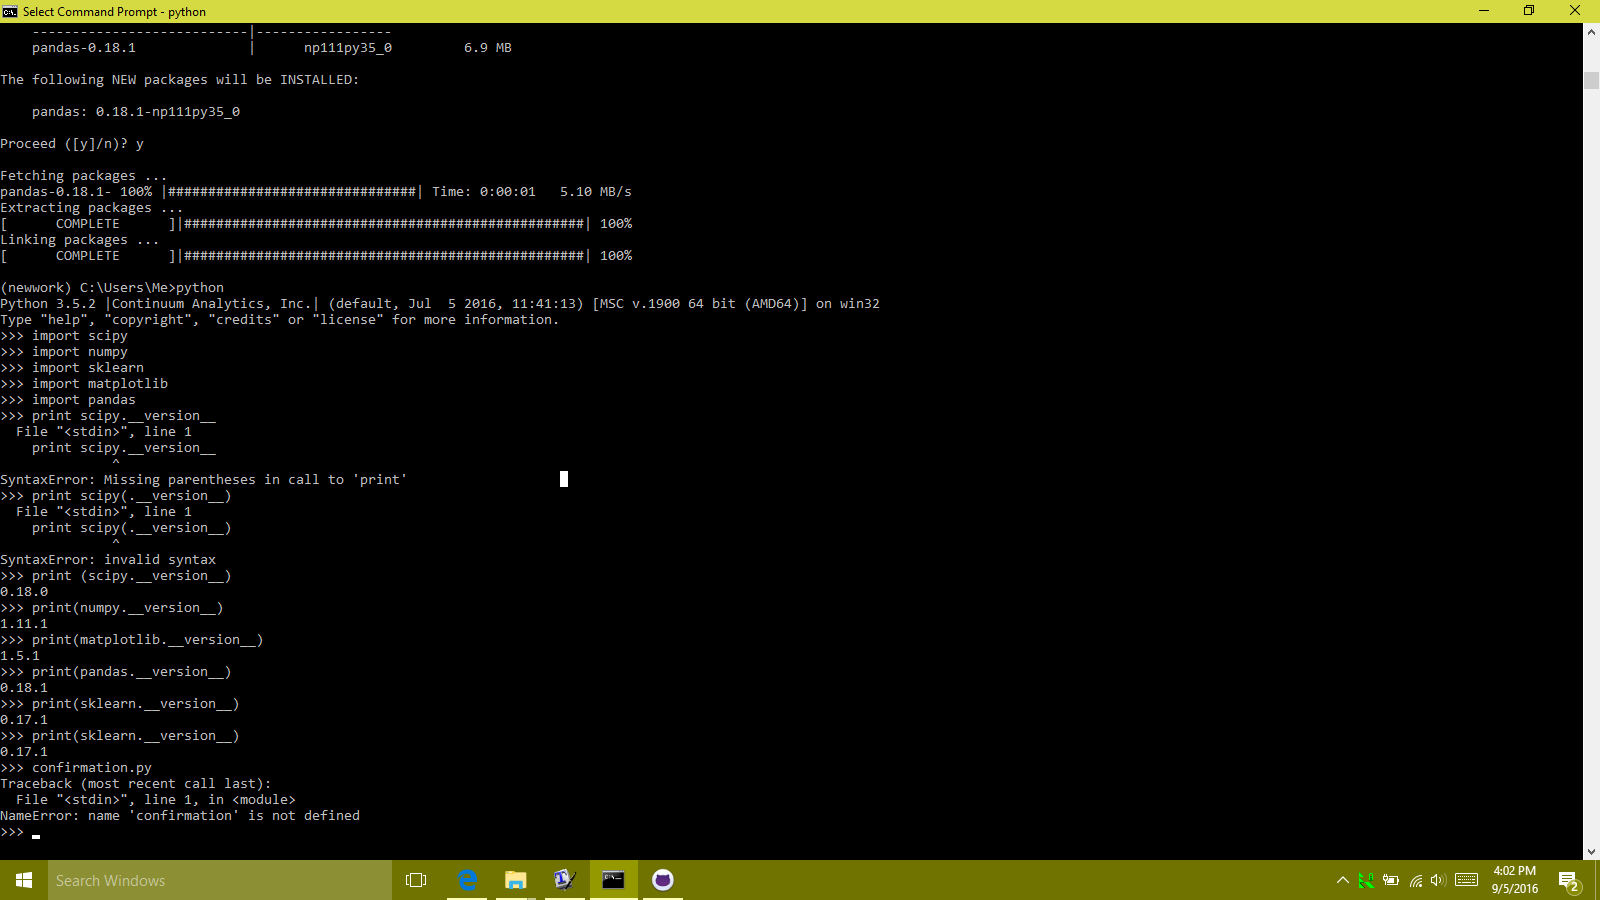
\includegraphics[width=\linewidth]{PythonConfirmation.png}
  \caption{Confirmation for Python.}
  \label{fig:PythonConfirm}
\end{figure}

\subsection{Soltution to Section 2.2}
GitHub repository is up. pablorp80 is added as a collaborator.the site can be found \href{http://wwwgithub.com/Gingerbreed/ArtificialIntelligence404}{here.}There's another screenshot from the collaborator page, Figure \ref{fig:CollabConfirm}

\begin{figure}
  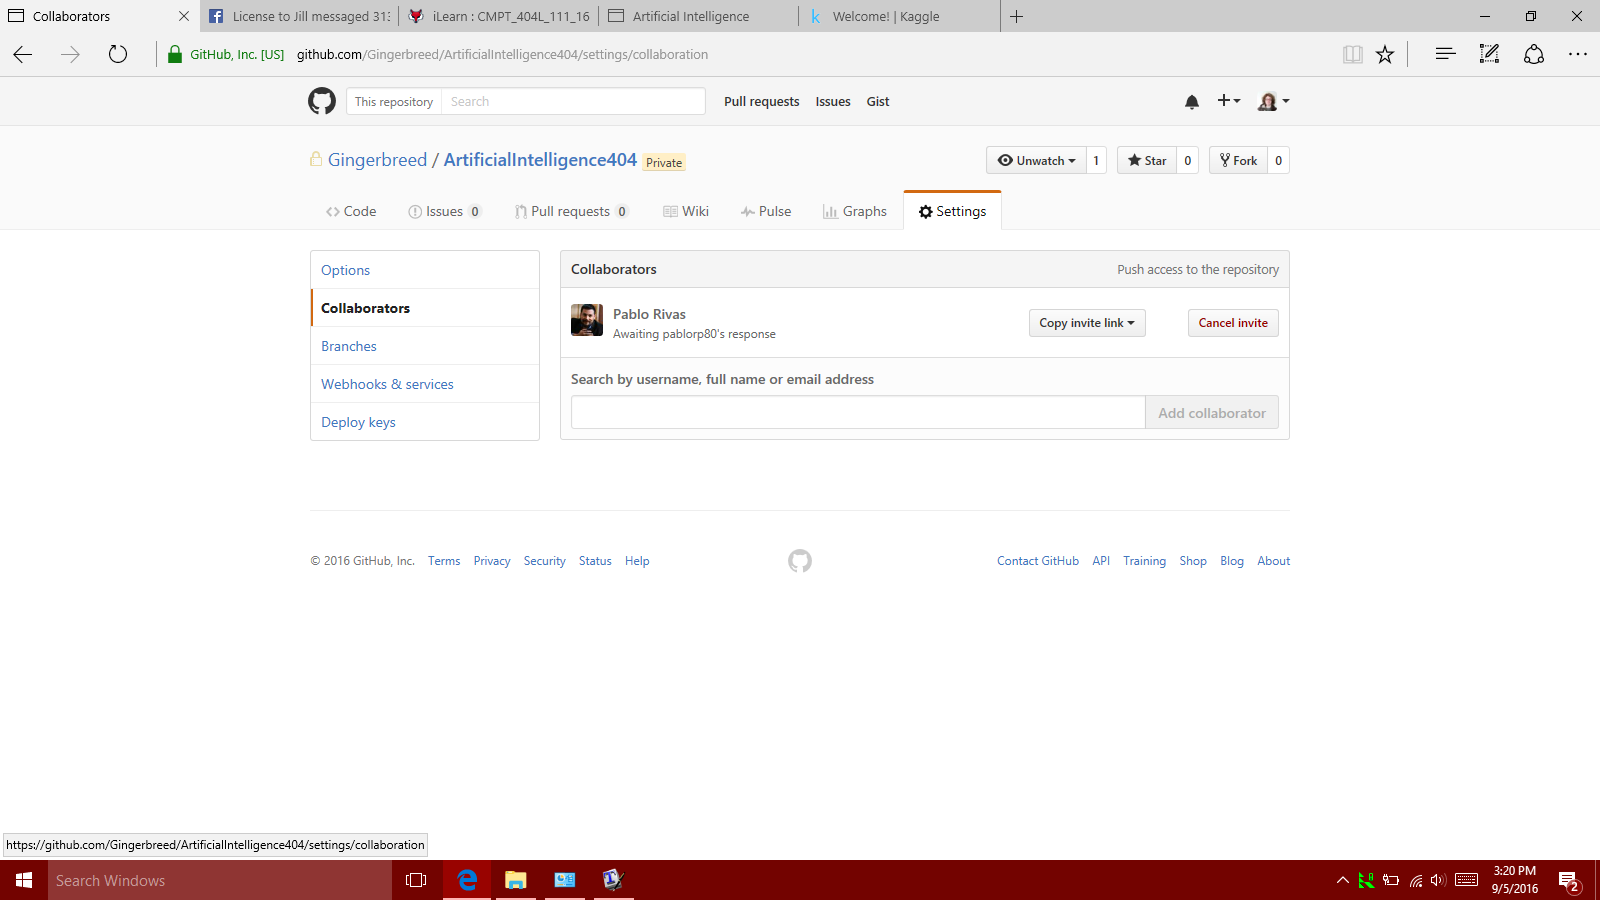
\includegraphics[width=\linewidth]{Collaborators.png}
  \caption{Confirmation for Collaborators.}
  \label{fig:CollabConfirm}
\end{figure}	

\subsection{Solution to Section 2.3}
Kaggle is up. My username is Gingerbreed. There is proof in Figure \ref {fig:Kaggle}.


\begin{figure}
  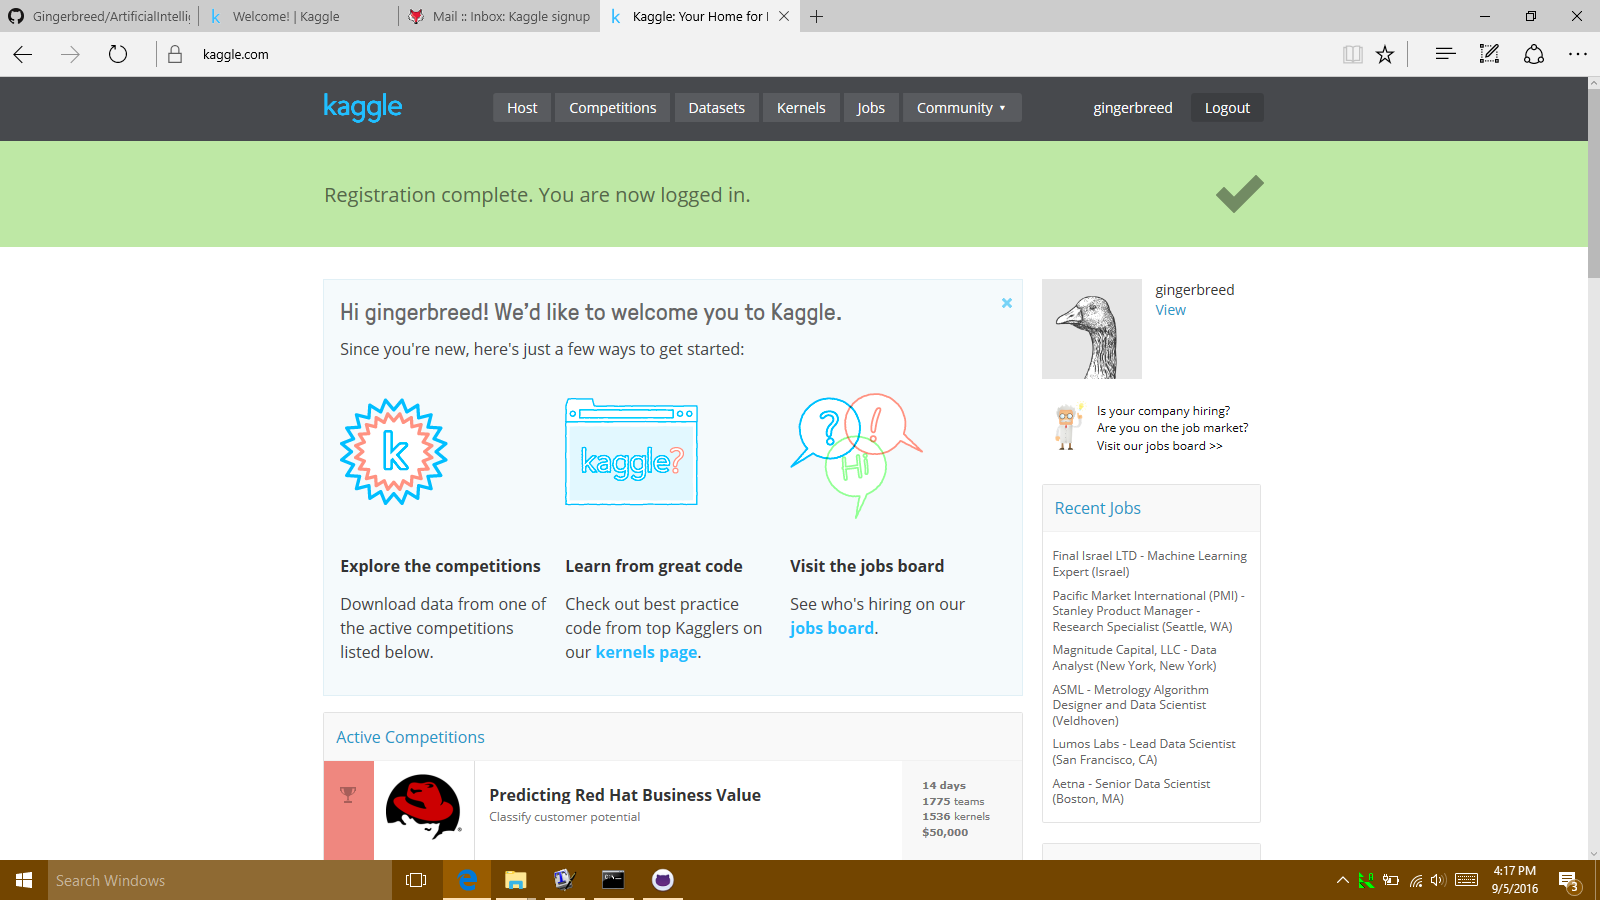
\includegraphics[width=\linewidth]{KaggleConfirm.png}
  \caption{Confirmation for Kaggle.}
  \label{fig:Kaggle}
\end{figure}

\section{Solution to Section 3}
No Deliverables.

\section{Solution to Section 4}
\subsection{Solution to Section 4.1}
The  x value that maximizes the function $-3x^2 + 24x -30$ can be found by setting the derivative to 0. The derivative of the function is $-6x + 24$. The 0 for the derivative is 4, meaning the maximum for the function $-3x^2 + 24x -30$ is 4.

\subsection{Solution to Section 4.2}
The partial derivative of a function is taking a function and deriving the specific variables. The partial derivative of the function $3x^3 -2xy^2+4y-8$ with respect to X is $9x^2 - 2y^2$. The partial derivative with respect to y (x1) is $-4xy+4$. or $-4 * (xy-1)$.


\subsection{Solution to Section 4.3a}
The matrices 
$\begin{matrix}
1 &4 &-3\\
2 &-1 &3
\end{matrix}$ and
$\begin{matrix}
-2 &0 &5\\
0 &-1 &4
\end{matrix}$ cannot be multiplied! The shapes of the matrices need to be reversed. An example is 3 by 2 and 2 by 3, but not 3 by 2 and 3 by 2. 

\subsubsection{Solution to Section 4.3b}
The multiplication of the two matrices in the first section requires the transverse of matrix A (the first one). Finding the transverse is done by flipping the rows and making them into columns. The transverse of matrix A $\begin{matrix}
1 &4 &-3\\
2 &-1 &3
\end{matrix}$  is the matrix
$\begin{matrix}
1 & 2 \\
4 & -1\\
-3 & 3
\end{matrix}$ The new matrix can now be multiplied with matrix B (3 by 2 and 2 by 3). This is done by crossing the rows and columns of the two matrices. 
the end result is $\begin{matrix}-2 & -2 & 13\\
-8 & 1 & 16\\
6 & -3 & -3\end{matrix}$
You can see how this is true by looking at Figure \ref {fig:Matrix}

\begin{figure}
  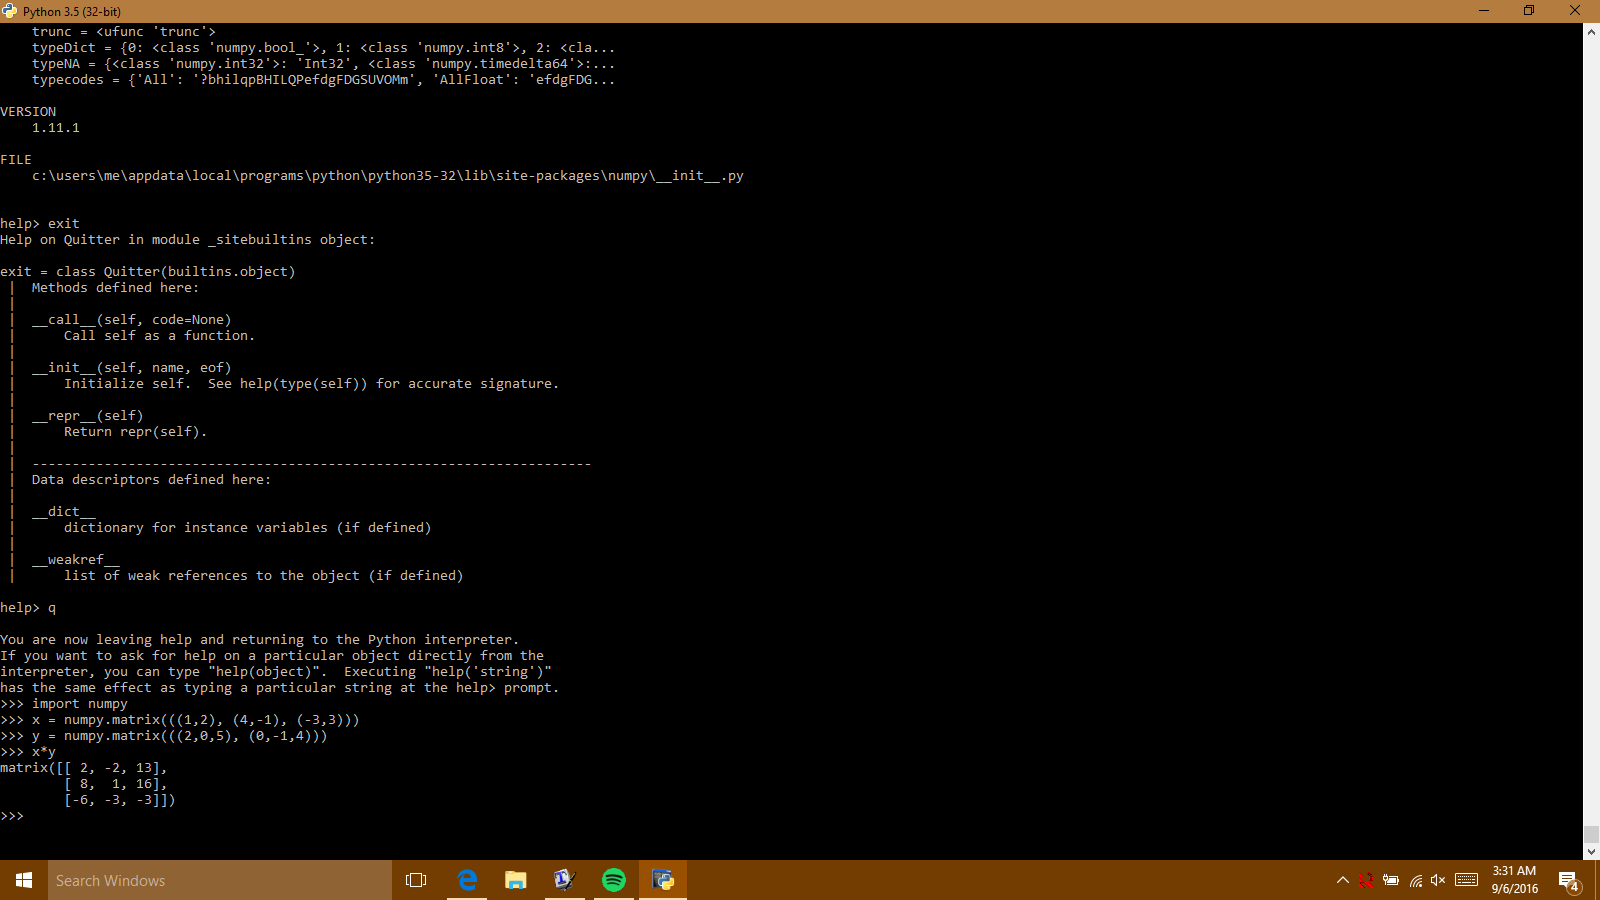
\includegraphics[width=\linewidth]{Matrix.png}
  \caption{Confirmation for problem 4.3b.}
  \label {fig:Matrix}
\end{figure}
\subsubsection{Solution to Section 4.3c}
This is a question for Graduate Students. I am not one of those.

\subsection{Solution to Section 4.4}
A Gaussian distribution is better known as a bell curve. It has a high point. A multivariate Gaussian is a higher version of a simple Gaussian. A Bernoulli is a distribution that will change depending on the input (usually with two cases). A binomial distribution uses the probability successes over trials. An exponential distribution is using a rate of change to predict success.

\subsection{Solution to Section 4.5}
This question is for Graduate Students. I am not one of those.

\subsection{Solution to Section 4.6}
Assuming that N is a probability distribution, the expected value of the distribution would be 2.

\subsection{Solution to Section 4.7a}
The answer to this question is 1.1. The minimum natural number is 0, so the arg min should be equal to 0. Since y is = to 1.1, x needs to be equal to 1.1 to achieve the minimum natural number.

\subsubsection{Solution to Section 4.7b}
The location of x* is as close to the y point as possible with one constraint. The x* must stay within the oval Z, because x* is still in the range of Z.

\subsection{Solution to Section 4.8a}
This is to verify that the closer you get to infinity, the upper limit of the function becomes 1. This can be seen by adding up the intervals. $e^-1 +e^-2 $ is closer to 1 than the two by themselves. but what about $e^0$, which should = 1? that gets cancelled by the other side, negative infinity.

\subsubsection{Solution to Section 4.8b}
The average (expected value) should be close to 0, if not zero. The mean requires you to add all the values and divide. $e^-1 +e^0+0 > e^-2 +e^-1 +e^0+0+0$ The zeroes in the equation are from the negatives. Considering the right side of this equation is only .3, the average for all of infinity would be 0. 

\subsubsection{Solution to Section 4.8c}
The variance here would be from 0(infinity) to 1(x=0), so the variance would be 1.

\subsubsection{Solution to Section 4.8d}
This would be a very small number, considering when y = 10 the function spits out $4.0* 10^-5$. I don't know exactly what the number would be, however.
 

\end{document}